%===============================================================================
% Template Name:      CDE Thesis Presentation template
% Template URI:       http://github.com/csaybar/cde-thesis/
% Description:        Starter Presentation template for CDE master thesis 
% Version:            1.1.1
% Author:             Johan Janse van Rensburg
% Modified by:        Cesar Aybar
% License:            MIT License
% License URI:        http://opensource.org/licenses/MIT
%===============================================================================


%=================================================
% theme and color
%=================================================
\documentclass[compress]{beamer}
\usepackage{amsfonts,amsmath,oldgerm}
\usetheme{sintef}
\usepackage{graphicx}
\usepackage{animate}
 	
\usetheme{Warsaw} % Themes http://www.hartwork.org/beamer-theme-matrix/
\usefonttheme[onlymath]{serif}



%=================================================
% packages and new commands
%=================================================
\usepackage[ruled, linesnumbered, vlined]{algorithm2e}
\usepackage{epsfig, subfigure, amssymb, multirow, algorithmic, amsmath}
\newcommand*{\superscript}[1]{\ensuremath{^{\rm #1}}}
\newcommand*{\subscript}[1]{\ensuremath{_{\rm #1}}}

%=================================================
% thesis details (first slide)
%=================================================
\title[{\sc How reliable are SEN2 cloud detection algorithms?} \hspace{0.8cm} \insertframenumber/\inserttotalframenumber]{{\sc How reliable are SEN2 cloud detection algorithms?}}
\subtitle{Global uncertainty estimation using Deep Kernel Learning.}
\author{\href{mailto:csaybar@gmail.com}{Cesar Luis Aybar Camacho}}
\institute{\textbf{Erasmus Mundus Joint Master Degree Programme \\ Copernicus Master in Digital Earth} \\ Specialization track GeoData Science}
\date{Vannes, France, 2022}


%=================================================
% start presentation
%=================================================
\begin{document}
	
%========================
% title page
%========================
\begingroup
\setbeamertemplate{headline}{}
\addtobeamertemplate{frametitle}{\vskip-1.7ex}{}
\begin{frame}
	\begin{center}
		\vspace{0.1cm}
		\includegraphics[scale=0.15]{images/logo.pdf}
	\end{center}
	\titlepage
\end{frame}
\endgroup

%========================
% your slides:
%========================
\section{Acknowledges}
\begin{frame}
	\frametitle{Acknowledge}
	\begin{center}
		\vspace{0.1cm}
		\includegraphics[scale=0.25]{images/acknowledge.pdf}
	\end{center}
\end{frame}


\section{Introduction}
\begin{frame}{What is a cloud?}
	\begin{center}
		\begin{figure}
			\centering
			\includegraphics[width=0.8\linewidth]{images/intro_fig00_0.png}
			\label{fig:introfig01}
	\end{figure}
	\vspace{20px}
	\textbf{A cloud is a mass of water drops or ice crystals suspended in the atmosphere.}	
	\end{center}
\end{frame}


\begin{frame}{What is a cloud?}
	\begin{center}
		\begin{figure}
			\centering
			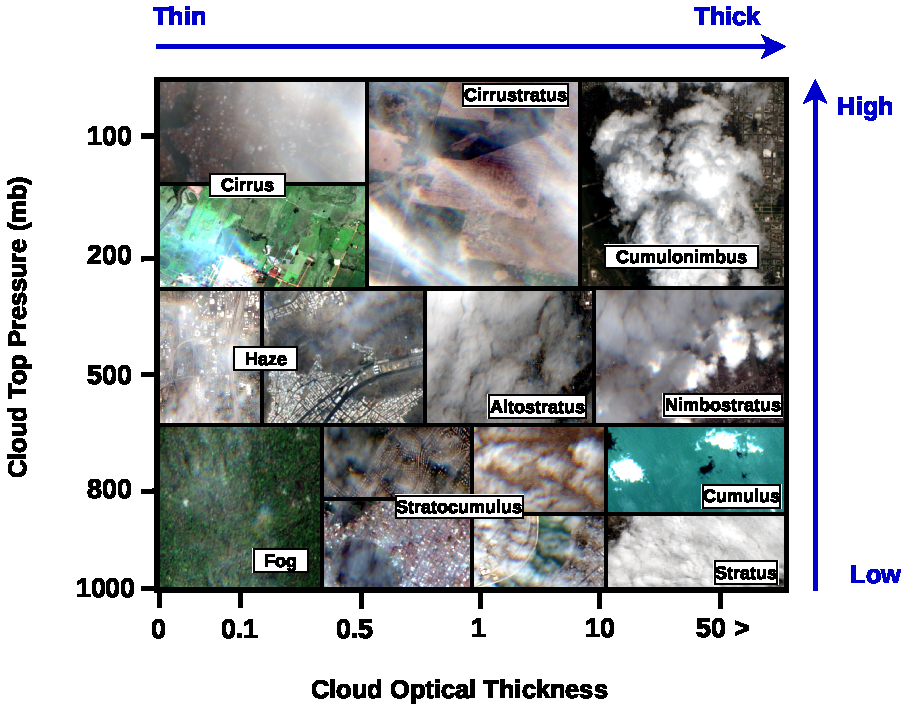
\includegraphics[width=0.7\linewidth]{images/cloud_types.pdf}
			\label{fig:introfig01}
		\end{figure}
		\textbf{A cloud is a mass of water drops or ice crystals suspended in the atmosphere.}	
	\end{center}
\end{frame}

\begin{frame}{What is a cloud?}
	\begin{center}
		\begin{figure}
			\centering
			\includegraphics[width=0.65\linewidth]{images/cloud_types2.png}
			\label{fig:introfig01}
		\end{figure}
		\textbf{Cloud classification - CloudSat (Ceccaldi, et al. 2020)}	
	\end{center}
\end{frame}

\begin{frame}{How do cloud cover algorithms work?}
	\begin{center}
		\begin{figure}
			\centering
			\includegraphics[width=0.85\linewidth]{images/intro_what_is_a_cloud.pdf}
			\label{fig:introfig01}
		\end{figure}
	\end{center}
\end{frame}


\begin{frame}{Context}
	\begin{center}
		\begin{figure}
			\centering
			\includegraphics[width=0.85\linewidth]{images/intro_fig01.png}
			\caption[fig:introfig01]{Geographical distribution reference cloud detection datasets for Sentinel-2 (Skakun et al. 2022).}
			\label{fig:introfig01}
		\end{figure}
	\end{center}
\end{frame}


\section{Data}
\begin{frame}
	\begin{center}
		\begin{figure}
			\animategraphics[width=0.55\linewidth,loop,autoplay]{10}{images/gif01/frame-}{0}{6}
		\end{figure}
		\textcolor{blue}{\href{https://cloudsen12.github.io/}{https://cloudsen12.github.io/}}
	\end{center}
\end{frame}


\begin{frame}{CloudSEN12 - Team <3}
	\begin{center}
		\begin{figure}
			\centering
			\includegraphics[width=1.0\linewidth]{images/dataset_team.png}
			{\caption*{CloudSEN12 team}}
			\label{fig:introfig01}
		\end{figure}
	\end{center}
\end{frame}


\begin{frame}{CloudSEN12 - Map}
	\begin{center}
		\begin{figure}
			\centering
			\includegraphics[width=0.85\linewidth]{images/intro_fig01.png}
			\caption[fig:introfig01]{Geographical distribution reference cloud detection datasets for Sentinel-2 (Skakun et al. 2022).}
			\label{fig:introfig01}
		\end{figure}
	\end{center}
\end{frame}

\begin{frame}{CloudSEN12 - Map}
	\begin{center}
		\begin{figure}
			\includegraphics[width=0.85\linewidth]{images/intro_fig04.png}
			\caption[fig:introfig04]{CloudSEN12 spatial distribution}
		\end{figure}
	\end{center}
\end{frame}


\begin{frame}{CloudSEN12 - Data preparation}
	\begin{columns}
		\begin{column}{0.6\textwidth}
			\begin{figure}
				\includegraphics[width=0.6\textwidth]{images/methodology01.png}
				\label{fig:introfig02}
			\end{figure}
		\end{column}
		\begin{column}{0.4\textwidth}
			\begin{itemize}
				\item Merging of different spatio-temporal datasets to use as predictors.
				\item Semi-automatic selection of ROIs (5090x5090 m.)
			\end{itemize}
		\end{column}
	\end{columns}
\end{frame}




\begin{frame}{CloudSEN12 - Data Selection}
	\begin{columns}
		\begin{column}{0.7\textwidth}
			\begin{figure}
				\includegraphics[width=1\textwidth]{images/methodology02.png}
				\label{fig:introfig02}
			\end{figure}
		\end{column}
		\begin{column}{0.3\textwidth}
			\begin{itemize}
				\item Each ROI have multiple IPs. We manually select five IPs considering the background, cloud type, and cloud coverage.
			\end{itemize}
		\end{column}
	\end{columns}
\end{frame}


\begin{frame}{CloudSEN12 - Labeling}
	\begin{columns}
		\begin{column}{0.7\textwidth}
			\begin{figure}
				\includegraphics[width=1\textwidth]{images/methodology03.png}
				\label{fig:introfig02}
			\end{figure}
		\end{column}
		\begin{column}{0.3\textwidth}
			\begin{itemize}
				\item Add to each IP the results of 6 different CD algorithms. In addition, each ROI counts with manual labeling that can be of type: high-quality, scribble, or no annotation.
			\end{itemize}
		\end{column}
	\end{columns}
\end{frame}


\begin{frame}{CloudSEN12 - Labels}
\begin{figure}
	\centering
	\includegraphics[width=0.7\linewidth]{images/labels01}
	\caption{}
	\label{fig:labels01}
\end{figure}
\end{frame}


\begin{frame}{CloudSEN12 - Labels}
	\begin{figure}
		\centering
		\includegraphics[width=0.7\linewidth]{images/labels02}
		\label{fig:labels01}
	\end{figure}
\end{frame}


\begin{frame}{CloudSEN12 - Labels}
	\begin{figure}
		\centering
		\includegraphics[width=0.7\linewidth]{images/labels03}
		\label{fig:labels01}
	\end{figure}
\end{frame}

\section{Methods}
\begin{frame}{Methodology}	
	\begin{enumerate}
		\item  The \textbf{cloudSEN12 high-quality dataset} is used only for this experiment $D$; pixel-by-pixel cloud masking is converted to cloud cover percentages in order to perform a regression task.
		\item The dataset of S2 L1C $\{x_1, x_2, ..., x_n\}$ and corresponding cloud cover percentages $\{y_1, y_2, ..., y_n\}$ is splitted in train ($D_{train}$), validation ($D_{val}$), and test ($D_{test}$) dataset.
		\item \textcolor{red}{\textbf{Experiment 01}}: Convolutional Neural Network (CNN) for regression.
	\end{enumerate}
\end{frame}



\begin{frame}{Methodology}	
	\begin{enumerate}
		\item  The \textbf{cloudSEN12 high-quality dataset} is used only for this experiment $D$; pixel-by-pixel cloud masking is converted to cloud cover percentages in order to perform a regression task.
		\item The dataset of S2 L1C $\{x_1, x_2, ..., x_n\}$ and corresponding cloud cover percentages $\{y_1, y_2, ..., y_n\}$ is splitted in train ($D_{train}$), validation ($D_{val}$), and test ($D_{test}$) dataset.		
		\item \textcolor{red}{\textbf{Experiment 02}}: CNN with a GP header layer.
		\begin{itemize}
			\item Residual CNN $f_\theta: x \rightarrow R^J$ with feature space dimensionality $J$ and parameters $\theta$.
			\item Exact GP header with parameters $\phi = \{l, s\}$ where $l$ and $s$ are kernel hyperparameters.			
		\end{itemize}		
	\end{enumerate}
\end{frame}


\begin{frame}{Methodology}
	\begin{enumerate}
		\item  The \textbf{cloudSEN12 high-quality dataset} is used only for this experiment $D$; pixel-by-pixel cloud masking is converted to cloud cover percentages in order to perform a regression task.
		\item The dataset of S2 L1C $\{x_1, x_2, ..., x_n\}$ and corresponding cloud cover percentages $\{y_1, y_2, ..., y_n\}$ is splitted in train ($D_{train}$), validation ($D_{val}$), and test ($D_{test}$) dataset.
		\item \textcolor{red}{\textbf{Experiment 03}}: Variational Deep Kernel Learning.
		\begin{itemize}
			\item Residual NN $f_\theta: x \rightarrow R^J$ with feature space dimensionality $J$ and parameters $\theta$.			
			\item Approximate GP header with parameters $\phi = \{l, s, \omega\}$ where $l$ and $s$ are kernel hyperparameters, $\omega$ GP variational parameters (including $m$ inducing point locations $Z$).
			\item Using a random subset of $p$ points of our training
			data, $X^{init} \subset X$, compute; \textbf{Initial inducing points:} Use found centroids as initial inducing point locations Z in GP. \textbf{Initial length scale:} set
			as 1.			
		\end{itemize}
	\end{enumerate}
\end{frame}


\begin{frame}{Experiment 01}
\begin{figure}
	\centering
	\includegraphics[width=1\linewidth]{images/method_01}
	\caption{}
	\label{fig:method01}
\end{figure}
\end{frame}


\begin{frame}{Experiment 02 - Gaussian processes}
\textbf{\large Definition}

A Gaussian process (GP) is a collection of random variables, any finite number of which have a joint Gaussian distribution.

\textbf{\large Nonparametric Regression Model}
Prior: $f(x) \sim \mathcal{G P}\left(m(x), k\left(x, x^{\prime}\right)\right)$, meaning $\left(f\left(x_{1}\right), \ldots, f\left(x_{N}\right)\right) \sim \mathcal{N}(\boldsymbol{\mu}, K)$, with $\mu_{i}=m\left(x_{i}\right)$ and $K_{i j}=\operatorname{cov}\left(f\left(x_{i}\right), f\left(x_{j}\right)\right)=k\left(x_{i}, x_{j}\right)$.
$$
\overbrace{p(f(x) \mid \mathcal{D})}^{\text {GP posterior }} \propto \overbrace{p(\mathcal{D} \mid f(x))}^{\text {Likelihood }} \overbrace{p(f(x))}^{\text {GP prior }}
$$
	
\begin{figure}
	\centering
	\includegraphics[width=0.75\linewidth]{images/gp01}
	\caption{}
	\label{fig:gp01}
\end{figure}
\end{frame}


\begin{frame}{Experiment 02 - Gaussian processes}
\begin{figure}
	\centering
	\includegraphics[width=0.75\linewidth]{images/gp02}
	\caption{}
	\label{fig:gp01}
\end{figure}
\end{frame}


\begin{frame}{Experiment 02 - Gaussian processes}
	\begin{figure}
		\centering
		\includegraphics[width=0.75\linewidth]{images/gp03}
		\caption{}
		\label{fig:gp01}
	\end{figure}
\end{frame}

\begin{frame}{Experiment 02 - Gaussian processes}
	\begin{figure}
		\centering
		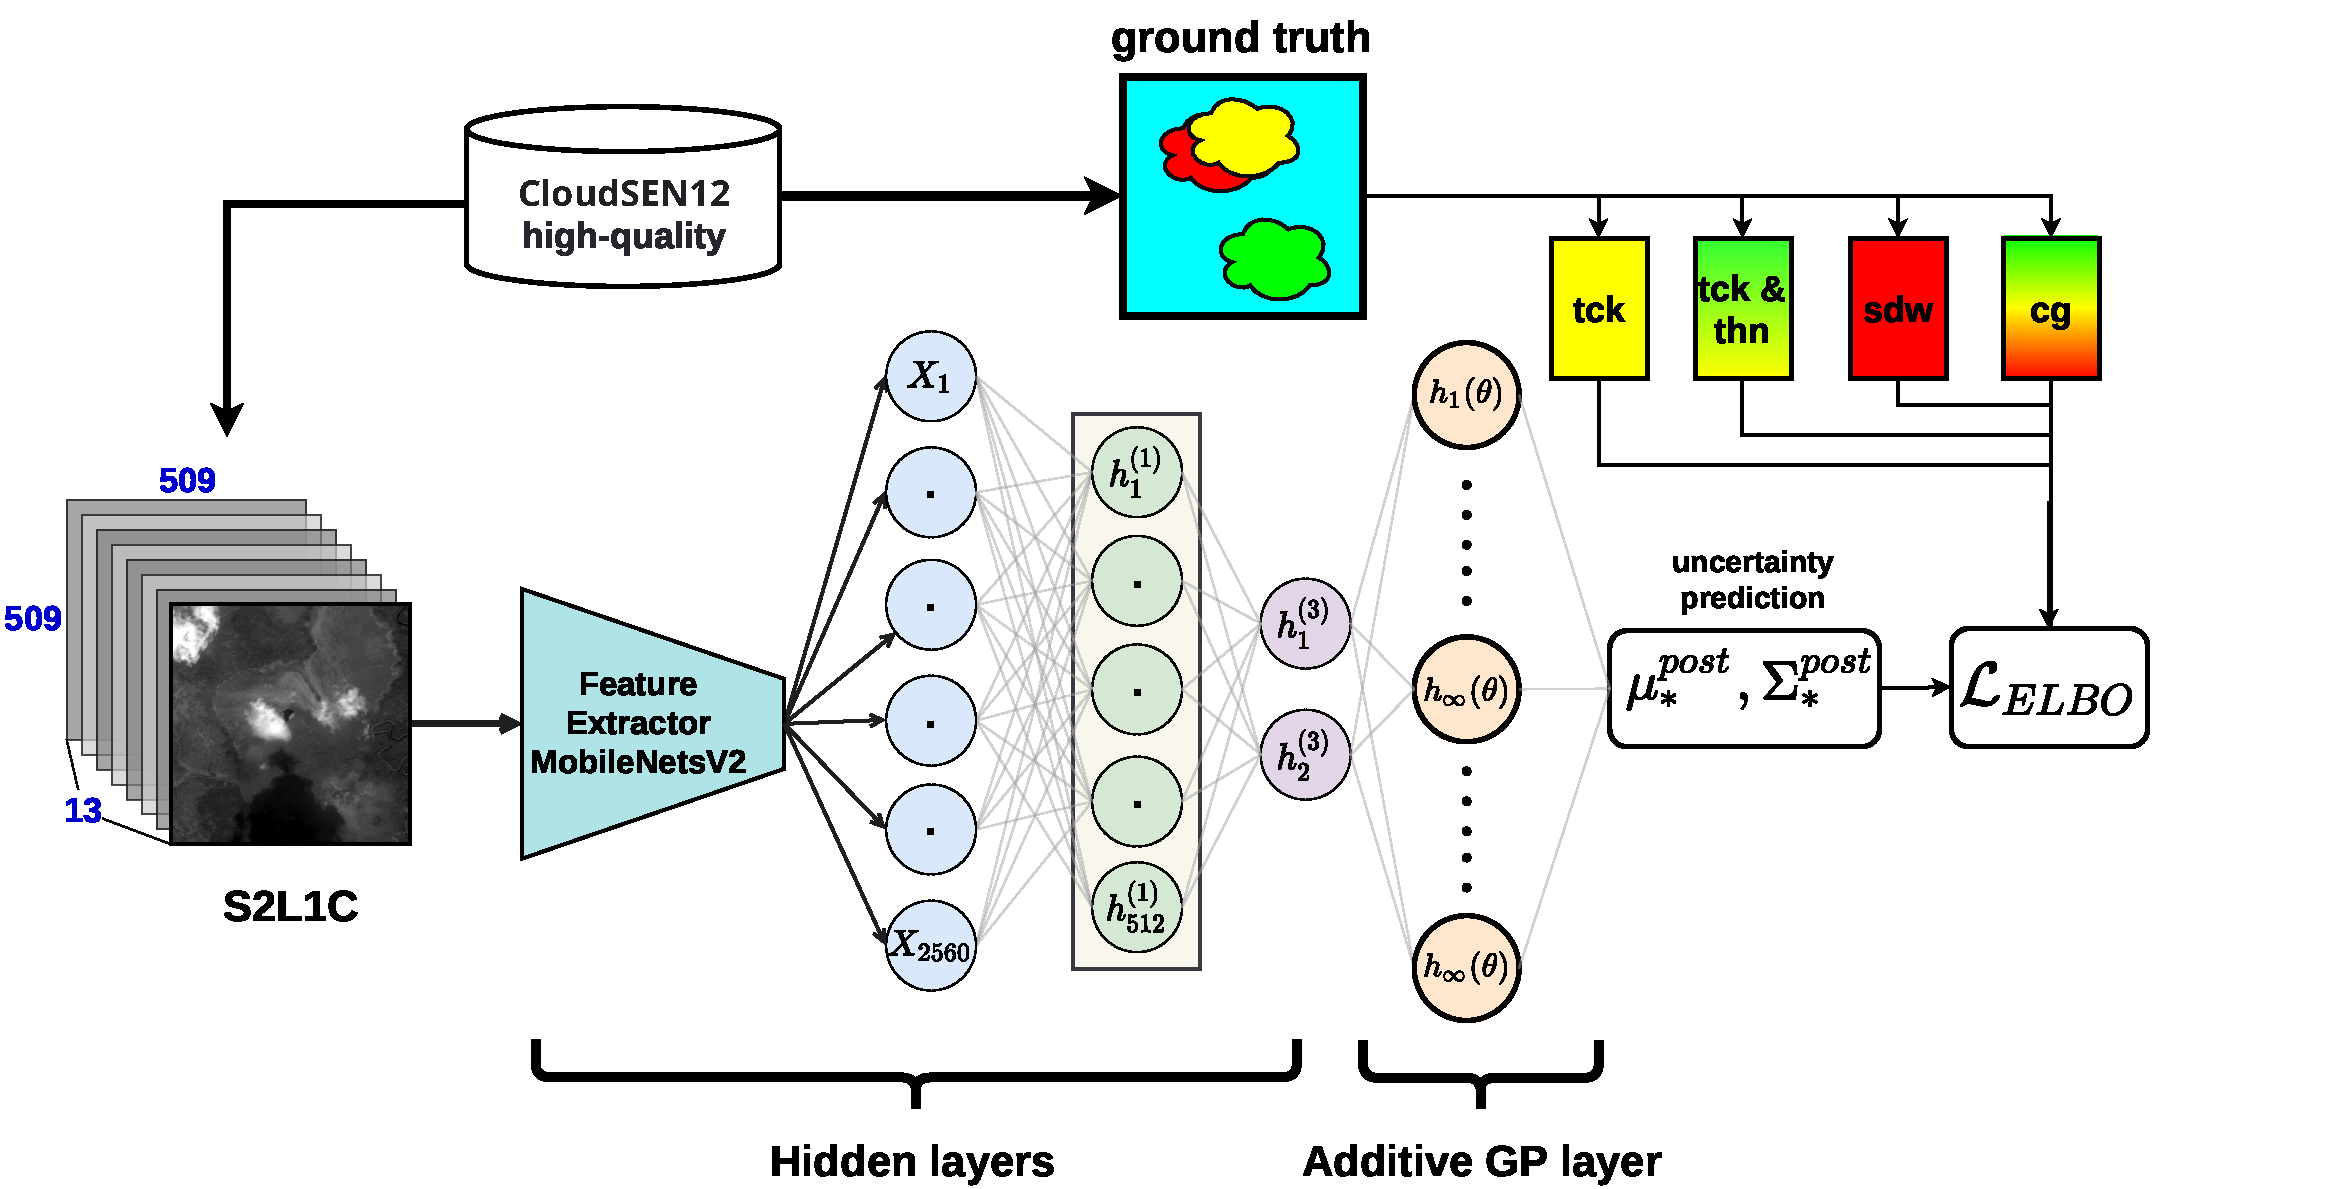
\includegraphics[width=1\linewidth]{images/metodology.pdf}
		\caption{}
		\label{fig:gp01}
	\end{figure}
\end{frame}



\begin{frame}{Experiment 03 - Stochastic Variational DKL}
	\begin{figure}
		\centering
		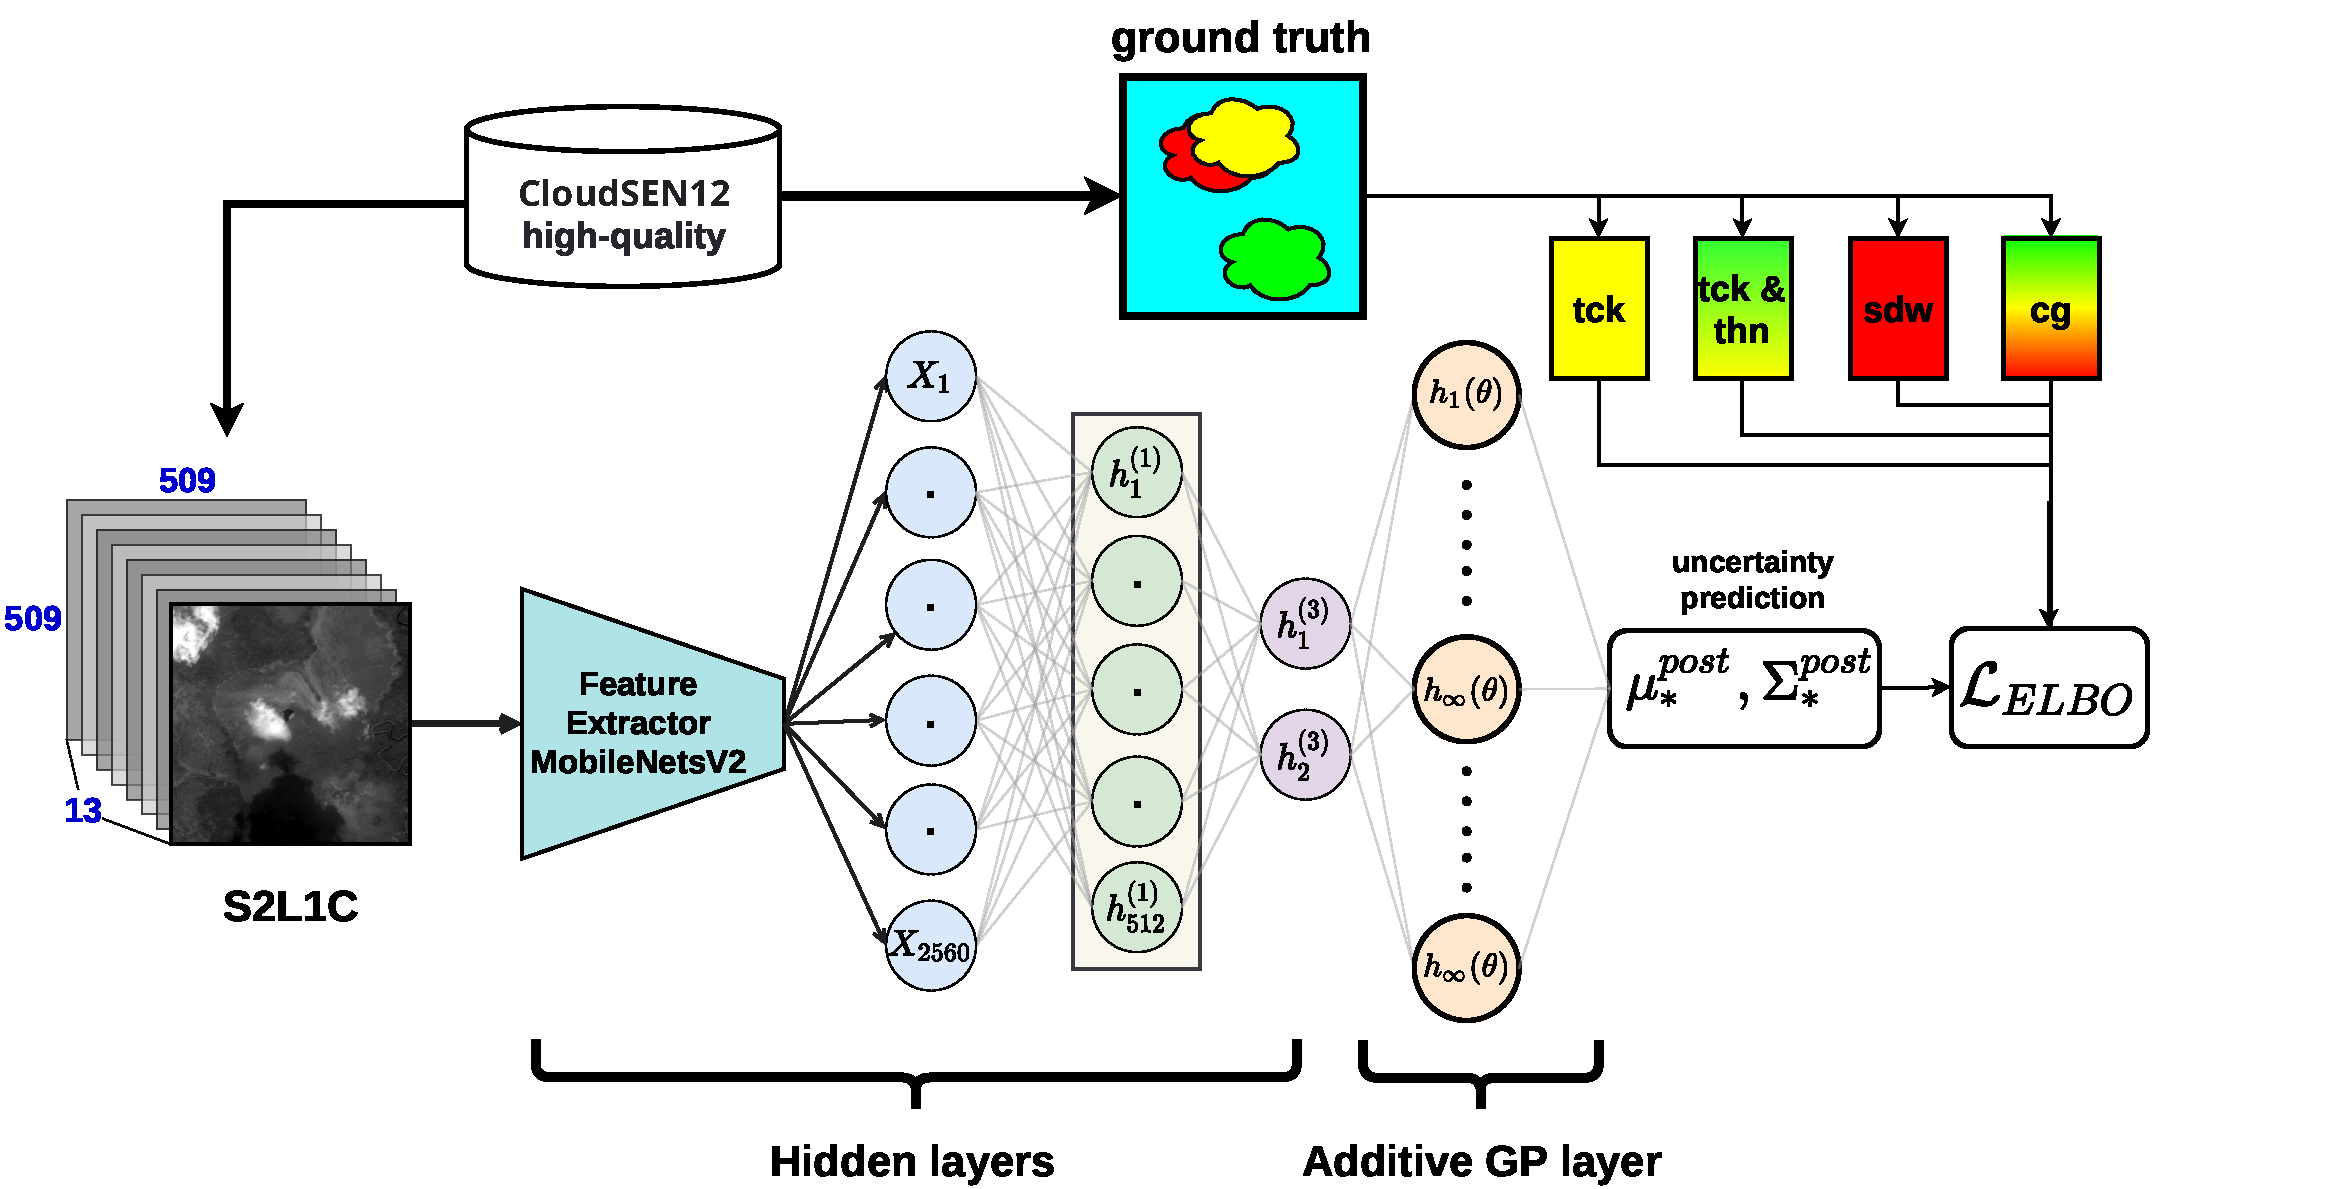
\includegraphics[width=1\linewidth]{images/metodology.pdf}
		\caption{}
		\label{fig:gp01}
	\end{figure}
\end{frame}


\section{Results}
\input{slides/results}

\section{Conclusions}
\input{slides/conclusions}

%========================
% bibliography
%========================
\input{slides/bib}

%=================================================
% end presentation
%=================================================
\end{document}